

\chapter{Обзор литературы} \label{review}
\section{Летательные аппараты мультироторного типа} \label{review_s1}

История развития летательных аппаратов мультироторного типа началась более ста лет назад, когда братья Бриджет и профессор Ричет создали конструкцию, которую назвали Гироплан №1 \cite{Leishman02, Leishman01}. Осенью 1907 года их гироплан вместе с пилотом на борту оторвался от земли менее чем на метр, продемонстрировав практическую возможность использования конструкции такого типа. С тех пор интерес исследователей к мультикоптерам постепенно возрастал и в настоящее время находится на очень высоком уровне, во многом благодаря развитию технологий производства комплектующих для аппаратов такого типа и значительному уменьшению габаритов и массы бортовой вычислительной техники и датчиков, необходимых для построения автономной системы управления. Из-за простоты конструкции, маневренности, относительной доступности и дешевизны особенной популярностью сейчас пользуются квадрокоптеры -- беспилотные летательные аппараты мультироторнного типа с четырьмя двигателями. Эти преимущества позволяют использовать такие аппараты как инструмент для отработки новых подходов к построению систем управления и их тестированию на практике. Этот факт закономерно привел к тому, что на текущий момент существует достаточно большое количество работ, посвященных управляемой динамике беспилотных летательных аппаратов такого типа, значительно отличающихся по поставленным в иследованиях целям, применяемым методам и полученным результатам. В ряде публикаций предлагаются некоторые модификации конструкции стандартного квадрокоптера, которые позволяют повысить летные характеристики беспилотного летательного аппарата (БЛА) и гарантируют некоторые другие преимущества перед квадрокоптерами стандартной конструкции. Ниже рассмотрены встречающиеся в современных публикациях основные подходы, посвященные проектированию систем управления как стандартных, так и модифицированных конструкций БЛА, в основе которых лежат ПИД-регуляторы, линейно-квадратичные регуляторы, скользящие режимы управления, адаптивное управление, робастное управление и другие методы современной теории управления.

\section{Конструкция и основные принципы движения квадрокоптера}

Основными элементами конструкции стандартного квадрокоптера являются корпус и четыре двигателя с прикрепленными к ним пропеллерами. В зависимости от взаимного расположения двигателей и собственных осей аппарата выделяют две стандартных схемы: \textit{cross}-схему и \textit{plus}-схему \cite{Bashi01} (см. рис. \ref{fig:cross_plus}).
\begin{figure}[h!]
	\centering
	\subfloat[Общий вид \textit{cross}-схемы]{%
		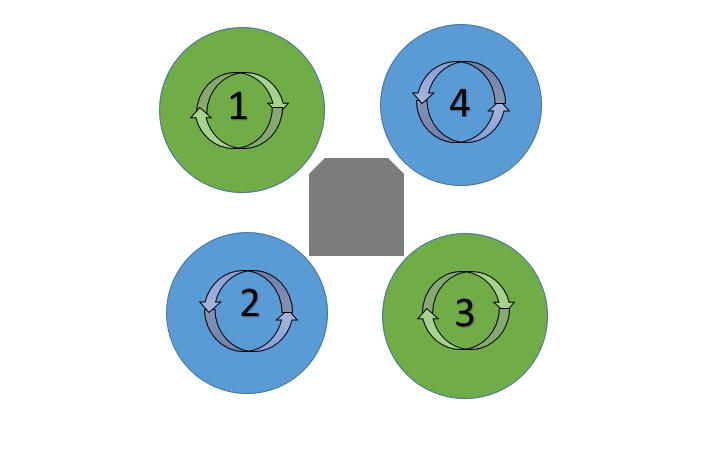
\includegraphics[width=0.44\columnwidth]{cross}%
	}
	\quad
	\subfloat[Общий вид \textit{plus}-схемы]{%
		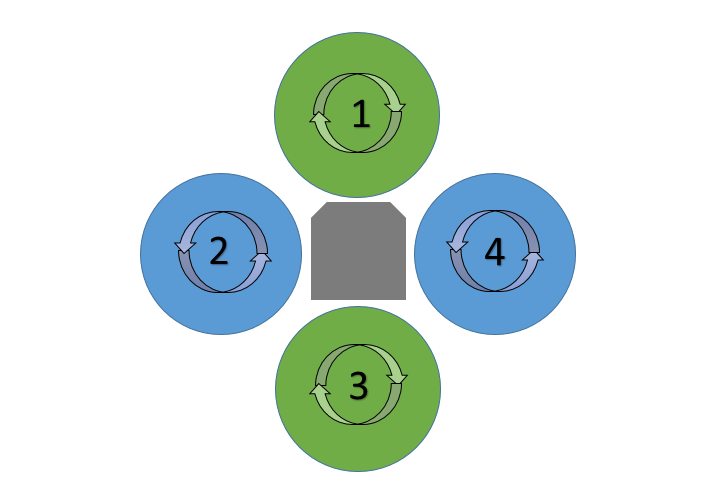
\includegraphics[width=0.44\columnwidth]{plus}%
	}
	\caption{ -- Основные схемы квадрокоптеров}
	\label{fig:cross_plus}
\end{figure}
Пропеллеры, расположенные на смежных лучах, вращаются в разные стороны, благодаря чему возможна стабилизация по углу рысканья, при этом тяга каждого двигателя направленна одинаково. Вертикальное движение аппарата обусловлено изменением общей тяги всех двигателей. Горизонтальное движение совершается за счет изменения направления вектора тяги вследствие наклона корпуса БЛА \cite{Salih01}. 

\section{Основные подходы к построению модели динамики квадрокоптера}
	
Обычно, поступательное движение малых беспилотных летательных аппаратов рассматривают в инерциальной системе координат (назовем ее {$I$}), связанной с поверхностью Земли. С учетом относительно небольших характерных расстояний и времен полета БЛА движением и кривизной поверхности Земли принебрегают.

Существуют два наиболее распространенных способа связать координатные оси с Землей: {$NED$} --  ось \textbf{$X_I$} направлена на север, ось \textbf{$Y_I$} -- на восток, а ось \textbf{$Z_I$} -- к центру Земли; {$ENU$} -- ось \textbf{$X_I$} направлена на восток, ось \textbf{$Y_I$} -- на север, а ось \textbf{$Z_I$} -- от центра Земли. Положение БЛА описывается радиус-вектором центра масс аппарата \bm{$r_I$}, записанном в выбранной инерциальной системе координат. Скорость определяется, как
\begin{equation} \label{eq:velocity}
\bm{v_I} = \dot{\bm{r}}.
\end{equation}

Корпус квадрокоптера в рамках задачи управления движением обычно считают твердым телом. Для описания ориентации объекта в пространстве используют связанную с телом систему координат $B$, начало которой совпадает с центром масс БЛА, а оси направлены по главным центральным осям инерции корпуса (см. рис. \ref{fig:quad_scheme}). Текущее положение базиса B относительно I может быть описано матрицей поворота $\bm{R}_{IB}$, в том смысле, что разложения произвольного вектора $\bm{x}$, записанного в этих базисах, связаны соотношением
\begin{figure}[h!]
	\centering
	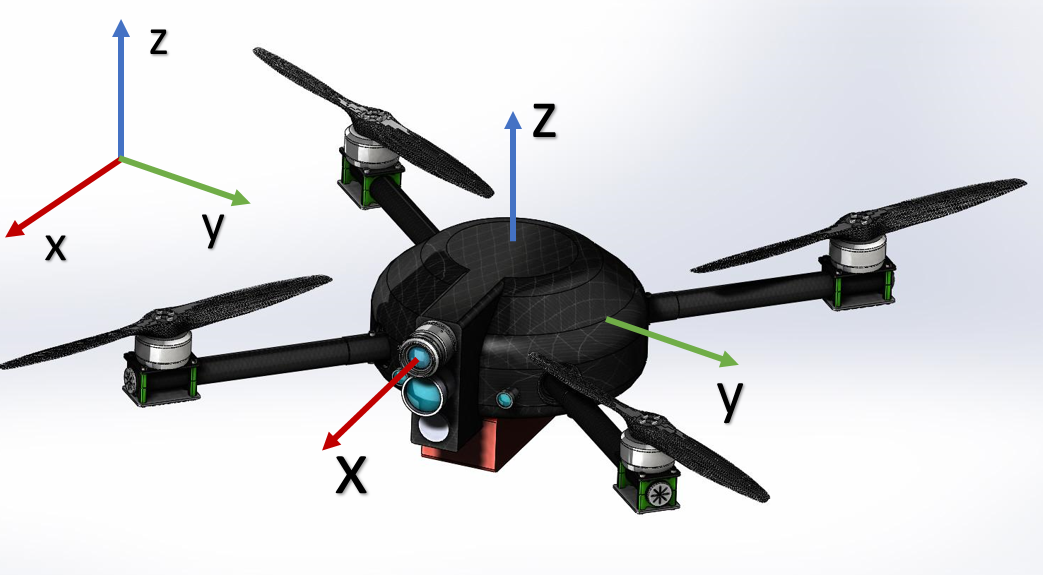
\includegraphics[width=0.9\columnwidth]{uavXYZ}
	\caption{ -- Квадрокоптер и системы кординат}
	\label{fig:quad_scheme}
\end{figure}
\begin{equation} \label{eq:rotmx}
\bm{x}_I = \bm{R}_{IB}\bm{x}_B.
\end{equation}
Матрица поворота связана с компонентами угловой $\bm{\Omega}_B$ скорости следующим соотношением
\begin{equation} \label{eq:angvel_rotmx}
\dot{\bm{R}}_{IB} = \bm{R}_{IB} [\bm{\Omega}_B]_{\times},
\end{equation}
где
\begin{equation} \label{eq:hat_operator}
[\bm{\Omega}]_{\times} =
\begin{bmatrix}
0            & -\bm{\Omega}^z   & \bm{\Omega}^y \\
\bm{\Omega}^z     & 0           &-\bm{\Omega}^x\\
-\bm{\Omega}^y    & \bm{\Omega}^x    & 0
\end{bmatrix}.
\end{equation}

Иногда для описания ориентации БЛА используют углы конечного поворота (иногда их называют углами Эйлера вне зависимости от последовательности), которые задают положение базиса B относительно базиса I через три  последовательных поворота вокруг осей связанной системы координат. Наиболее часто используются так называемые самолетные углы: последовательные повороты вокруг оси $Z_B$ на угол $\psi$, $Y_B$ на угол $\theta$, $X_B$ на угол $\phi$ будут определять углы рысканья, крена и тангажа. Им соответствует матрица поворота

\small
\begin{equation*} \label{eq:eul_to_rotmx}
\begin{aligned}
\bm{R} =
&\begin{bmatrix}
c(\psi)c(\theta) & c(\psi)s(\theta)s(\phi) - s(\psi)c(\phi) & c(\psi)s(\theta)c(\phi) + s(\psi)s(\phi) \\
s(\psi)c(\theta) & s(\psi)s(\theta)s(\phi) - c(\psi)c(\phi) & s(\psi)s(\theta)c(\phi) - c(\psi)s(\phi) \\
-s(\theta)         & c(\psi)s(\phi)                                 & c(\psi)c(\phi)\\
\end{bmatrix},
\end{aligned}
\end{equation*}
\normalsize
где для произвольного аргумента $x$ обозначим $c(x) = cos(x)$, $s(x) = sin(x)$. Обратное преобразование:
\begin{equation} \label{eq:rotmx_to_eul}
\begin{aligned}
&\psi  = \arctan\left( { - \frac{{{{\bm{R}}_{13}}}}{{{{\bm{R}}_{23}}}}} \right),
\\
\vspace{3mm}
\\
&{\theta  = \arccos  ({{{\bm{R}}_{33}}} )}
\\
\vspace{3mm}
\\
&\varphi  = \arctan\left( {\frac{{{{\bm{R}}_{31}}}}{{{{\bm{R}}_{32}}}}} \right)
\end{aligned}
\end{equation}

Помимо матриц и углов конечного поворота для описания ориентации часто используются кватернионы \cite{Amelkin01} -- четырехмерные гиперкомплексные числа, которые можно представить в виде формальной суммы скалярной и векторной частей
\begin{equation} \label{eq:quat_def}
Q = q_0 + \bm{q}.
\end{equation}
Для кватернионов определены операции сопряжения
\begin{equation} \label{eq:quat_dual}
\tilde{Q} = q_0 - \bm{q}
\end{equation}
и умножения
\begin{equation} \label{eq:quat_mult}
Q \circ P = q_0 p_0 - (\bm{q} \cdot \bm{p})
+ q_0 \bm{p} + p_0 \bm{q} + \bm{q} \times \bm{p}
\end{equation}
Кватернион ориентации  $q_{IB}$ определяет положение собственного базиса $B$ относительно базиса $I$ в том смысле, что разложения произвольного вектора $\bm{x}$, записанного в этих базисах, связаны соотношением
\begin{equation} \label{eq:quat}
\bm{x}_I = q_{IB} \circ \bm{x}_B \circ \tilde{q}_{IB}.
\end{equation}
Угловая скорость и кватернион ориентации связаны уравнением Пуассона
\begin{equation} \label{eq:puasson}
\dot{q}_{IB} = \frac{1}{2} {q}_{IB} \circ \bm{\Omega}_B.
\end{equation}
Кватернион ориентации эквивалентен матрице поворота
\begin{equation} \label{eq:quat_to_rotmx}
\bm{R} = ({q_0}^2 - \bm{q}^T \bm{q}) E_{3 \times 3} + 2 \bm{q}^T \bm{q} - 2 {q_0} [\bm{q}]_{\times},
\end{equation}
где $E_{n \times n}$ -- едичная матрица размерности $n$.
Его компоненты могут быть получены из углов Эйлера
\begin{equation}
\begin{aligned}
&{q_0} = \cos \frac{\theta }{2}\cos \frac{{\varphi  + \psi }}{2},
\\
\vspace{3mm}
\\
&{q_1} = \sin\frac{\theta }{2}\cos \frac{{\varphi  - \psi }}{2},
\\
\vspace{3mm}
\\
&{q_2} =  - \sin \frac{\theta }{2}\sin\frac{{\varphi  - \psi }}{2},
\\
\vspace{3mm}
\\
&{q_3} = \cos \frac{\theta }{2}\sin \frac{{\varphi  + \psi }}{2}.
\end{aligned}
\end{equation}

Движение центра масс БЛА определяется силами гравитации, аэродинамического сопротивления и тягой пропеллеров.
Иногда в моделях могут присутствовать и другие возмущения, например, учитывающие динамику полезной нагрузки \cite{Lim01}.
В их отсутствии уравнения для движения центра масс БЛА имеют вид
\begin{equation} \label{eq:common_traslational_motion}
m \ddot{\bm{r}} = \bm{F}_g + \bm{F}_{aero} + \bm{F}_{thr}.
\end{equation}
Основными параметрами, определяющими движение центра масс БЛА, являются общая масса {$m$} конструкции, ускорение свободного падения \bm{$g$}, плотность среды {$\rho_{air}$}, аэродинамические свойства корпуса аппарата и пропеллеров. Сила тяжести определяется выражением

\begin{equation} \label{eq:gravity_force}
\bm{F}_g = m\bm{g}.
\end{equation}

Аэродинамические свойства корпуса БЛА определются площадью лобового сечения корпуса аппарата {$S_{\perp}$} и аэродинамическими константами. Выражение для аэродинамической силы можно записать, как \cite{Biard01}

\begin{equation} \label{eq:aerodynamic_force}
\bm{F}_{aero} = - \frac{1}{2} \rho_{air} C S_{\perp} |\dot{\bm{r}}| \dot{\bm{r}}.
\end{equation}

Такая модель позволяет учитывать ветер \cite{Bannwarth01}. Форма корпуса стандартных квадрокоптеров позволяет пренебрегать подъемной аэродинамической силой, которая обычно не рассматривается при описании движения таких БЛА.

Силу тяги пропеллеров обычно определяют через квадрат их оборотов $\tilde\omega$ и аэродинамический коэффициент $k$ \cite{Falconi01}

\begin{equation} \label{eq:thrust_force}
\bm{F}_{thr} = \sum_{i=1}^{4}{ { k \tilde\omega^2_i \bm{z}_i}.}
\end{equation}
Здесь $\bm{z}_i$ -- ось вращения $i$-того пропеллера.
 
Вращательное движение корпуса БЛА определяется моментами сил, которые создают двигатели с пропеллерами и гироскопическим моментом самого корпуса

\begin{equation} \label{eq:common_rotational_motion}
\sum_{i=1}^{4}{\bm{\tau}_{Bi}} = \bm{J}_B\dot{\bm{\Omega}}_B + \bm{\Omega}_B \times  \bm{J}_B{\bm{\Omega}_B},
\end{equation}
где $\bm{J}_B$ -- тензор инерции корпуса БЛА, записанный в его главных осях.
Внешний момент, действующий на пропеллер, связывают с квадратом его оборотов с помощью аэродинамического коэффициента $b$ \cite{Ryll01}

\begin{equation} \label{eq:rotor_ext_torque}
\bm{\tau}_{Bi}^{ext} = -b \tilde{\omega}^2_i \bm{z_i}.
\end{equation}
Также модель может включать в себя аэродинамические моменты \cite{Solovev01}.

При синтезе контура управления квадрокоптера стандартной конструкции в качестве компонентов вектора управления выбирают обороты его двигателей или некоторые их функции \cite{Sharifi01, Luukkonen01, Bemporad01}.  С учетом выражений (\ref{eq:thrust_force}), (\ref{eq:rotor_ext_torque}) удобно сформировать вектор управляющих воздействий из квадратов скоростей вращения пропеллеров

\begin{equation} \label{eq:common_control_vector}
u_i = \tilde{\omega}_i^2.
\end{equation}
Конкретные выражения для компонент зависят от рассматриваемой схемы квадрокоптера и способа нумерации его двигателей.
 
\section{Различные варианты постановки задачи управления}
Цели управления БЛА могут быть сформулированы по-разному,
начиная от приведения его центра масс в некоторое наперед заданное статичное положение
\cite{Huynh01, Yuskin01}
или обеспечения требуемой ориентации и высоты
\cite{Domingos01, Wang01, Gheorghita01, Lukmana01, Zabko01},
и заканчивая наблюдением за внешними объектами
\cite{Rodriguez01, Kendall01, Razinkova01}
и построением пространственных формаций
\cite{Ali01, Zhao01, Preiss01}.
 
Увеличение размерности вектора управляющего воздействия, например, за счет изменения угла атаки лопастей пропеллера \cite{Cutler01, Cutler02}  или изменения ориентации двигателей относительно корпуса \cite{Sridhar02, Kumar02}, позволяет расширить маневренные возможности БЛА и усложнить поставленные перед ними задачи. Например, в работе \cite{Ryll02} в качестве задачи управления выбрано отслеживание аппаратом произвольной траетории в пространстве при независимом управлении ориентацией его корпуса. Подобная задача решена в исследовании \cite{Kaufman01} для БЛА с шестью двигателями с использованием пропеллеров с переменной геометрией. Применение таких пропеллеров для экстремальных маневров, включая фигуры высшего пилотажа, показали в работе \cite{Cutler02}.
 
Далее мы детально рассмотрим те техники и подходы, которые применяются для решения поставленных задач управления. 

\section{Управление с использованием ПИД-регуляторов}

ПИД-регуляторы широко используются в системах управления БЛА.
Такая популярность связана с их простой и понятной реализацией, а также рядом важных особенностей, таких, как способность устранять статические ошибки благодаря интегральной составляющей и прогнозировать состояние управляемой системы с помощью дифференциальной составляющей  \cite{Astrom01}.
Помимо этого, алгоритмы управления, использующие ПИД-регуляторы, обычно не требуют больших вычислительных ресурсов.
Однако, существует ряд проблем при применении этой техники к построению систем управления квадрокоптероми, включающие нелинейности, связанные с математической моделью и неточностями моделирования динамики.
Поэтому применение ПИД-регуляторов для квадрокоптеров может ограничить их производительность \cite{Zulu01}.

Работа ПИД-регулятора основана на вычислении текущей ошибки положения в координатном пространстве $\bm{e}$, которая является разностью целевого состояния и оценки текущего состояния. Затем, управляющее воздействие вычисляется, как
\begin{equation} \label{eq:pid_common}
\bm{u}(t) = K_P \bm{e}(t) + K_I\int_0^t \bm{e}(t) dt + K_D \frac{d\bm{e}(t)}{dt},
\end{equation}
где $K_P$, $K_I$ и $K_D$ -- пропорциональный, интегральный и дифференциальный коэффициенты соответственно.

В работе \cite{Li01} применена схема с использованием ПИД-регулятора для управления положением и ориентацией БЛА.
Рассматриваемый аппарат спроектирован по \textit{plus}-схеме.
Ориентация аппарата описана углами Эйлера.
Динамическая модель включает в себя все основные силы и моменты (\ref{eq:common_traslational_motion}) - (\ref{eq:rotor_ext_torque}), действующие на аппарат, без каких-либо дополнительных возмущений.
Вектор состояния включает в себя скорость центра масс БЛА, углы его ориентации и их производные по времени.
Компоненты вектора управления являются функциями от квадратов скоростей вращения пропеллеров; первая компонента отвечает за общую тягу всех двигателей, остальные три -- за моменты сил, действующие вдоль собственных координатных осей.
Используя метод малых возмущений, авторы линеаризуют модель в окрестности текущего положения, находят передаточные функции по всем каналам управления, которые затем используют для построения модели.
Параметры модели соответствуют небольшому летательному аппарату с массой чуть больше одного килограмма.
В работе подобраны коэффициенты ПИД-регулятора, при которых БЛА удается стабилизировать свою позицию и ориентацию около целевой точки.
Далее в работе описан прототип летательного аппарата, реализующий предложенные алгоритмы.
Проведены летные испытания, ошибка по углам ориентации не превысила пяти градусов.

Последовательное применение ПД-регуляторов для управления положением и ориентацией используется в работе \cite{Mellinger01}. Рассматриваемый апарат также спроектирован по \textit{plus}-схеме.
Ориентация описывается углами Эйлера и с помощью матриц поворота.
Приведены некоторые аргументы в пользу использования простой модели двигателей
(\ref{eq:thrust_force}, \ref{eq:rotor_ext_torque}).
Компоненты вектора управляющего воздействия отвечают за тягу и моменты, действующие на корпус БЛА со стороны приводов:
\begin{equation} \label{eq:mellinger_control_vector}
	\begin{aligned}
	\bm{u} =
	\begin{bmatrix}
	k & k & k & k\\
	0 & kL & 0 & -kL\\
	-kL & 0 & k	L & 0\\
	b & -b & b & -b
	\end{bmatrix}
	\begin{bmatrix}
	\omega^{2}_{1}\\
	\omega^{2}_{2}\\
	\omega^{2}_{3}\\
	\omega^{2}_{4}
	\end{bmatrix},
	\end{aligned}
\end{equation}
где $L$ -- расстояние от центра масс БЛА до осей вращения роторов.
Вектор состояния включает в себя позицию, ориентацию, а также линейную и угловую скорости аппарата
\begin{equation} \label{eq:mellinger_state}
\bm{x} = [\bm{r}_I, \phi, \theta, \psi, \bm{v}_I, \bm{\Omega}_B].
\end{equation}

Целью управления является отслеживание аппаратом траектории в пространстве и заданного угла рысканья. Авторы показывают, что модель является дифференциально плоской \cite{Belinskaya01, Nieuwstadt01} относительно выхода
\begin{equation} \label{eq:mellinger_flat_output}
\bm{\sigma} = (\bm{r},\psi)^T,
\end{equation}
то есть вектор состояния (\ref{eq:mellinger_state}) и вектор управляющих воздействий (\ref{eq:mellinger_control_vector}) может быть записан, как функция выхода  (\ref{eq:mellinger_flat_output}) и конечного числа его производных. Данный факт позволяет в дальнейшем строить оптимальные траектории в пространстве вектора выхода.

Синтезирован двухуровненвый контур управления. На первом уровне вычисляется ошибка позиционирования БЛА и используется ПД-регулятор для определения вектора целевой тяги квадрокоптера:
\begin{equation} \label{eq:mellinger_pos_err}
\bm{e}_r = \bm{r}^{0} - \bm{r},
\end{equation}
\begin{equation} \label{eq:mellinger_vel_err}
\bm{e}_v = \bm{v}^{0} - \bm{v},
\end{equation}
\begin{equation} \label{eq:mellinger_pos_reg}
\bm{F}^0 = K_r \bm{e}_r + K_v \bm{e}_v + m \bm{g} + m \ddot{\bm{r}}^0,
\end{equation}
где $\bm{r}^{0}$, $\bm{v}^{0}$, $\ddot{\bm{r}}^{0}$, $\bm{F}^{0}$ -- целевые координата, скорость, ускорение и общая сила тяги аппарата, а $K_r$ и $K_v$ -- некоторые положительно определенные матрицы.
Затем, положив $ || \bm{F}^{0} || > 0$
(что равносильно запрету на свободное падение БЛА),
авторы вычисляют первую компоненту вектора управляющих воздействий (\ref{eq:mellinger_control_vector}),
как
\begin{equation} \label{eq:mellinger_u1}
u_1 = \bm{F}^{0} \cdot \bm{z}_B,
\end{equation}
и определяют целевую ориентацию при известном угле рысканья из условия
\begin{equation} \label{eq:mellinger_Rdes}
\bm{R}_{IB}^0 [0,0,1]^T = \frac{\bm{F}^{0}}{||\bm{F}^{0}||}.
\end{equation}
На основе ошибки ориентации
\begin{equation} \label{eq:mellinger_eR}
\bm{e}_R = \frac{1}{2}
\Big[
(\bm{R}_{IB}^0)^T 	\bm{R}_{IB} -
(\bm{R}_{IB})^T \bm{R}_{IB}^0
\Big]_\vee,
\end{equation}
где оператор $[...]_\vee$ является обратным преобразованием к (\ref{eq:hat_operator}), и ошибки по угловой скорости вычисляются оставшиеся компоненты вектора управляющих воздействий
\begin{equation} \label{eq:mellinger_att_reg}
[u_2, u_3, u_4]^T = K_R \bm{e}_R + K_{\Omega} \bm{e}_{\Omega}.
\end{equation}
Затем авторы вычисляют значения оборотов каждого из двигателей на основе выражения (\ref{eq:mellinger_control_vector}).
	
В заключительной части работы рассматривается вопрос построения траекторий. Авторы строят кусочно-полиминиальную кривую через набор точек маршрута, минимизируя интеграл квадрата нормы второй производной ускорения центра масс аппарата и интеграл квадрата нормы второй производной угла его рысканья. Затем  авторы показывают, как можно локализовать некоторые участки траектории в прямоугольной области, для того, чтобы избежать их пересечений с возможными препятствиями.

Производительность алгоритмов демонстрируется в натурном эксперименте. Траекторией БЛА является окружность, скорость аппарата превышает два с половиной метра в секунду, а углы крена тангажа достигают сорока градусов. Ошибка позиционирования не превышает пятнадцати сантиметров, однако ошибка ориентации авторами не приводится. Важной особенностью работы является учет нелинейной природы динамики квадрокоптера при синтезе контура управления. Это позволяет сохранять устойчивость управления при значительных отклонениях корпуса аппарата по углам тангажа и рысканья.

Исследование относительной эффективности применения ПИД регулятора для стабилизации ориентации корпуса квадрокоптера проводят авторы работы \cite{Bouabdallah01}. Кроме стандартных возущений, в модели присутствуют выражения для динамики бесколлекторных двигателей. Для синтеза контура управления авторы принебрегают гироскопическими эффектами со стороны двигателей с пропеллерами, упрощают и линеаризуют модель в окрестности точки соотвествующей неподвижному зависанию БЛА в воздухе. Ошибка ориентации, равная разнице целевого и текущего положения, записанных в углах Эйлера, подается на вход ПИД-регулятора, затем вычисляется вектор управления. Проведены вычислительные эксперименты и эксперименты на тестовом стенде. Авторы отмечают хорошую производительность алгоритмов управления, принимают во внимание эффекты, возникающие из-за более подробного моделирования динамики роторов и отмечают необходимость быстрого реагирования приводов робота на управление.

Затем происходит синтез второго контура управления, в основе которого лежит линейно-квадратичный регулятор (ЛК-регулятор, ЛКР) и сравнение полученных результатов.
	

\section{Управление с использованием ЛК-регуляторов}

Линейно-квадратичный регулятор -- один из видов оптимальных регуляторов, который применяется в линейных системах вида
\begin{equation} \label{eq:linear_dyn_system}
\dot{\bm{x}} = A\bm{x} + B\bm{u}
\end{equation}
и  использует квадратичный функционал вида
	\begin{equation} \label{eq:lqr_cost_func}
	F = \int_0^{\infty}{(\bm{x}^T Q \bm{x} + \bm{u}^T R \bm{u})} dt
	\end{equation}
в качестве критерия оптимальности. Управление, минимизируещее функционал \eqref{eq:lqr_cost_func}, имеет вид \cite{Letov01}
	\begin{equation} \label{eq:lqr_control_law}
	\bm{u} = -R^{-1} B^T P \bm{x},
	\end{equation}
где $P$ находится из решения уравнения Риккати
	\begin{equation} \label{eq:riqatty}
	A^T P + P A - P B R^{-1} B^T P + Q = -\dot{P}.
	\end{equation}
Такой подход относительно распространен при проектировании систем управления роботов, в том числе и мультикоптеров \cite{Baklanov01, Muhhamid01, Argentim01} и позволяет оптимизировать некоторые параметры движения. Однако, как отмечают авторы некоторых работ, производительность ЛК-регуляторов сильно зависит от полноты математической модели и точности определения параметров динамики системы \cite{Kim01, Joukhadar01}. Рассмотрим некоторые работы более подробно.

Сравнение эффективности различных подходов для синтеза системы управления квадрокоптером приведено в работе \cite{Bouabdallah01}. Для того чтобы применить линейно-квадратичного регулятор, авторы линеаризуют модель в окрестности текущего положения, затем решают уравнение Рикатти и находят компоненты вектора управляющего воздействия.
Численные и стендовые эксперименты показывают, что такой подход обеспечивает лучшую стабилизацию аппарата в пространстве, чем при применении ПИД-регулятора, что может быть следствием использования более полной модели динамики БЛА при синтезе ЛК-регулятора.

Подобным образом проектируют систему управления квадрокоптером авторы работы \cite{Reyes-Valeria01}. Модель аппарата исполнена по \textit{plus}-схеме. Кинематика вращательного движения представлена в кватернионном описании. Вектор состояния содержит положение центра масс аппарата, его скорость, кватернион ориентации и угловую скорость. Динамика аппарата, помимо стандартных сил и моментов, содержит аэродинамические моменты, действующие на корпус БЛА. Для линеаризации модели авторы выбирают точку неподвижного зависания квадрокоптера и затем строят ЛК-регулятор, который определяет оптимальную траекторию в его координатном пространстве. Из-за нестабильного поведения системы вдали от целевой траектории авторы синтезируют второй, независимый регулятор, который заменяет первый в случае значительных отклонений от целевых параметров движения. Работоспособность контура управления иллюстрируется численными экспериментами. Графики демонстрируют сходимость траектории к целевой, при этом углы ориентации в процессе движения не приводятся.

В работе  \cite{Minh01} продемонстрирован подход к решению проблемы большой чуствительности систем управления на основе ЛК-регулирования к точности модели и текущих параметров движения. Авторы расширяют модель системы \eqref{eq:linear_dyn_system}, добавив возмущения $G \bm{w}$ и шум измерений $\bm{v}$
\begin{equation} \label{eq:linear_dyn_system_noisy}
\begin{aligned}
&\dot{\bm{x}} = A\bm{x} + B\bm{u} + G \bm{w}\\
&\bm{y} = C \bm{x} + \bm{v}.
\end{aligned}
\end{equation}
Затем для оценки состояния используется расширенный фильтр Калмана и применяется линейно-квадратичное гауссовское (ЛКГ) управление с интегральным действием. Численные эксперименты демонстрируют возможность стабилизировать аппарат в некоторой точке. Преимущество ЛКГ подхода заключается в отсутствии необходимости очень точно оценивать текущее состояние объекта управления.

%% SLIDE MODE
\section{Управление с использованием скользящего режима}

Скользящий режим (\textit{sliding mode}) -- один из видов робастного управления, при котором управляющие воздейтвие на объект обеспечивает его движение в пределах выбранной поверхности в фазовом пространстве, не позволяя выбранным параметрам выходить за пределы допустимых, чем обеспечивается устойчивость такого движения.
При смещении траектории объекта за пределы поверхности включается активное управление, кторое возвращает его на одну из допустимых траекторий.
К преимуществам этого подхода можно отнести отсутствие необходимости линеаризовывать уравнения движения и малая чуствительность к изменениям параметров динамики управляемого объекта, что весьма актуально для синтеза систем управления мультироторными роботами.
Однако, использование такого подхода требует особой осторожности, так как неучтенные эффекты в работе исполнительных органов системы управления могут привести к вибрациям, потере энергии и другим нежелательным эффектам \cite{Utkin01}.

Синтез системы управления с использованием метода скользящего режима включает в себя два основных шага. На первом шаге необходимо выбрать поверхность в фазовом пространстве, движение в окрестности которой обеспечит сходимость состояния системы к целевому. Для системы
\begin{equation} \label{eq:slide_mode_system}
\dot{\bm x} = f(\bm x, t) + g( \bm x, t) \bm u,
\end{equation}
где $\bm x$ -- вектор состояния, $\bm u$ -- вектор управляющих воздействий, в качестве такой поверхности обычно выбирают \cite{Samir01}
\begin{equation} \label{eq:slide_mode_S}
S(\bm x) = \bm e + \lambda \dot{\bm e},
\end{equation}
где $\bm e$ -- рассогласование текущего и целевого состояния, $\lambda > 0$ -- некоторая константа. На втором шаге происходит поиск закона управления, который приводит и сохраняет траекторию системы в окрестности заданной на предыдущем шаге поверхности.
\begin{equation} \label{eq:slide_mode_on_S}
S(\bm x,t) = 0.
\end{equation}
Такой подход применяется как для квадрокоптеров \cite{Stevanovic01, Lebedev01, Xu01}, так и для летающих роботов другой конструкции \cite{Yih01, Zhu01}. Рассмотрим некоторые примеры.

В работе \cite{Samir01} скользящий режим применяется для синтеза управления квадрокоптера \textit{cross}-конфигурации.
Модель (\ref{eq:common_traslational_motion}, \ref{eq:common_rotational_motion}, \ref{eq:rotor_ext_torque}, \ref{eq:thrust_force}) дополнена динамикой бесколлекторных двигателей.
Авторы синтезируют двухуровневый контур управления, последовательно применяя скользящий режим для положения и ориентации объекта. При этом сначала, используя величину общей тяги квадрокоптера, стабилизируется высота аппарата, а затем второй регулятор обеспечивает необходимые для заданного горизонтального движения углы крена и тангажа. Численные эксперименты показали способность предложенных алгоритмов стабилизировать аппарат в точке, удаленной от исходной на расстоянии чуть более 3 метров, за время около 10 секунд.

Скользящий режим также используется в работе \cite{Runcharoon01}. Здесь, подобно \cite{Samir01}, синтезируется двухуровневый контур управления, однако \textit{sliding mode} регулятор отвечает только за ориентацию корпуса БЛА, когда как ПД-регулятор -- за его положение. Выражения для компонент вектора управляющего воздействия авторы определяют, полагаясь на результаты \cite{Slotine01}. Основным отличием, при этом, является использование более «гладкого» управления в окрестности целевой поверхности $S(\bm x)$. Вычислительные эксперименты демонстрируют, что данный шаг значительно сокращает время сходимости  ориентации корпуса БЛА к целевой. 

Отдельное внимание стоит уделить исследованию \cite{Sumantri01}, где использовалась нелинейная поверхность $S(\bm x)$, что позволило значительно повысить устойчивость БЛА к внешним возмущениям.

%% Robust Control
\section{Робастное управление}

В реальных задачах часто бывает невозможно с абсолютной точностью определить модель рассматриваемого объекта или параметры его динамики.
В случае необходимости гарантировать качество управления и оценить влияние таких неточностей на движение управляемого объекта используют обширный функционал теории робастного управления.
При описании системы с помощью передаточных функций неопределенный объект можно описать как
\begin{equation} \label{eq:robust_ctrl_obj}
H(s, q) = \frac{A(s, q)}{B(s, q)}, q \in Q,
\end{equation}
где $A(s, q)$ и $B(s, q)$ -- неопределенные полиномы, коэффициенты которых зависят от $q \in Q$ \cite{Polyak01}. 

Такой подход может оказаться весьма полезен при рассмотрении управляемой динамики
мультироторных летающих роботов, параметры которой могут изменяться в известных пределах, в том числе из-за использования разной полезной нагрузки или постепенного износа пропеллеров. Среди примеров использования теории робастного управления для проектирования систем управления БЛА можно отметить работы \cite{Lee02, Borisov01, Petranevsky01, Bai01, Tony01}. Рассмотрим содержание последней.

После некоторых упрощений, авторы формулируют модель динамики квадрокоптера как 
\begin{equation} \label{eq:Tony_dyn}
\ddot{\bm x} = f(\bm x) + g( \bm x) \bm u + d(t),
\end{equation}
где вектор состояния $\bm x$ составлен из высоты и ориентации аппарата, представленной углами Эйлера, а возмущение $d(t)$ является неизвестной нелинейной и гладкой функцией времени. Цель управления -- асимптотическая сходимость центра масс БЛА к целевой траектории. Для выполнения поставленной задачи авторы вводят некоторые ограничения, например, модуль возмущения $d(t)$, а также первой и второй его производной ограничены некоторыми известными значениями. Подобные ограничения также сформулированы для параметрически заданой целевой траектории $\bm x_d(t)$ и других параметров модели. В результате исследователям удается синтезировать контур управления, работоспособность которого подтверждена численными экспериментами, где БЛА стабилизируется в окрестности заданной точки, при этом авторы отмечают, что возмущения при этом соответствуют относительной ошибке измерения массы от 20\% до 50\%.

%% Feedback Linearization
\section{Метод линеаризации обратной связью}

Метод линеаризации обратной связью применяют для нелинейных систем вида
\begin{equation} \label{eq:feedback_linearization_system}
\begin{aligned}
&\dot{\bm x} = f(\bm x) + g(\bm x) \bm u\\
&\bm y = h(\bm x),
\end{aligned}
\end{equation}
где $\bm x$ -- вектор состояния, $\bm u$ -- вход системы, $\bm y$ -- ее выход.
Суть метода состоит в поиске преобразования 
\begin{equation} \label{eq:feedback_linearization_transform}
\bm z = T(\bm x),
\end{equation}
и закона управления вида
\begin{equation} \label{eq:feedback_linearization_control}
\bm u = \alpha(\bm x) + \beta(\bm x) \bm v,
\end{equation}
где $\bm v$ -- новый вход системы , которые преобразуют нелинейную систему \eqref{eq:feedback_linearization_system} в эквивалентную линейную \cite{Slotine01}. Метод достаточно широко используется как для управления отдельными мультироторными роботами \cite{Chang01, Freddi01}, так и в области группового управления БЛА \cite{Mahmood01}. Рассмотрим некоторые примеры подробнее.

Воспользоваться методом линеаризации обратной связью для синтеза системы управления квадрокоптером удалось в работе \cite{Roza01}. Рассматривается квадрокоптер \textit{plus}-конфигурации. Авторы используют стандартную модель динамики БЛА такой конструкции (\ref{eq:common_traslational_motion}, \ref{eq:common_rotational_motion}, \ref{eq:rotor_ext_torque}, \ref{eq:thrust_force}), исключив силу аэродинамического сопротивления, при этом пояснив, что планируют добавить в модель это и другие возмущения в следующих работах. Постановка задачи требует асимптотической сходимости траектории центра масс БЛА к целевой, при которой функции его текущей скорости и угла рысканья также имеют асимптотическую сходимость к заданным значениям, которые, в свою очередь, зависят от смещения аппарата вдоль траектории. В вычислительном эксперименте в качестве траектории авторы выбрали плоскую окружность радиусом 10 метров и продемонстрировали принципиальную возможность выполнять летное задание для скоростей от 3 м/с до 15 м/с.

В работе \cite{Kanatnikov} рассматривается упрощенная модель движения квадрокоптера, где отсутсвует сила аэродинамического сопротивления и некоторые другие, не очень значительные эффекты.
Затем по отдельности рассматривается движение БЛА в горизонтальной и вертикальной плоскости.
Показано, что дифференцирование уравнений горизонтального движения квадрокоптера позволяет привести систему к каноническому виду 
\begin{equation*}
\begin{bmatrix}
&x\\ &y
\end{bmatrix} ^{IV}
=
P + Q \bm{u},
\end{equation*}
что позволяет синтезировать контур управления.

Исследование относительной эффективности метода линеаризации обратной связью приведено в работе \cite{Lee01}. Показано, что в сравнении с некоторыми другими подходами, данный метод обладает большей чувствительностью к шуму измерений и неточностям модели. Авторы делают вывод, что синтез контура управления с использованием метода линеаризации обратной связью можно эффективно применять совместно с другими алгоритмами, чтобы уменьшить влияние возмущений различной природы.

%% 
\section{Адаптивное управление}

Адаптивное управление -- широкий класс алгоритмов, позволяющих проектировать систему управления способной изменять параметры или структуру регулятора в зависимости от изменения параметров управляемого объекта или внешних возмущений.
Применение подобных алгоритмов для БЛА может быть обусловлено изменчивостью параметров динамики во время полета, например вследствие значительного снижения заряда батареи или наличия аэродинамических возмущений вблизи горизонтальной поверхности. Помимо этого, как удтверждают некоторые авторы, применение алгоритмов адаптивного управления позволяет не учитывать некоторые параметры динамики мультикоптеров \cite{Belyavskiy01}. Адаптивное управление к БЛА применяется, например, в \cite{Dydek01, Mu01, Bara01}.

В исследовании \cite{Bara01} рассматривается квадрокоптер стандартной конструкции, выполненный по \textit{cross}-схеме. Ориентация представленна углами Эйлера. Синтезирован двухуровневый контур управления, на первом уровне применяется регулятор на основе скользящего режима для управления горизонтальным положением БЛА. На втором уровне используется адаптивный регулятор для управления выделенной из модели полностью управляемой подсистемой, вектор состояния которой составлен из ориентации и общей тяги БЛА. Рассмотрено два подхода к построению адаптивного управления -- первый использует ошибку текущего положения и ориентации для оценки параметров динамики объекта, второй дополнительно использует разницу между измеренным и оцененным выходами управления. Комбинированный подход показал хорошую производительность в условиях полной неопределенности для ключевых параметров динамической модели.

Применение адаптивного управления для стабилизации движения квадрокоптера со смещающимся во времени центром масс рассмотрено в исследовании \cite{Palunko01}. Авторы применили линеаризацию обратной связью с последующим применением ПД-регулятора и показали, что такое управление неспособно справиться со стабилизацией движения БЛА. Затем применен аддитивный адаптивный компонент системы управления, с помощью которого оценивалось смещение центра масс аппарата и происходила коррекция рассчета управляющего вектора.

%% BACKSTAPPING
\section{Управление с использованием метода декомпозиции}

Метод декомпозиции (\textit{backstapping}) -- рекурсивный алгоритм, основанный на разбиении динамической системы на набор подсистем и поочередной стабилизации каждой из них. Метод активно применяется для мультироторных роботов \cite{Pota01, Chen01, Jung01, Huo01}.

В работе \cite{Madani01} показано, что алгоритм не является вычислительно затратным и способен справляться с возмущениями, однако чувствителен к точности в оценках параметров модели. Основная идея применения метода декомпозиции в исследовании состоит в том, чтобы стабилизировать систему в два этапа. Сначала осуществляется управление горизонтальным положением аппарата с помощью виртуального входа, использующего в качестве компонент некоторые функции от углов рысканья и тангажа. Затем осуществляется управление ориентацией БЛА  посредством изменения скорости вращения роторов.

\section{Оптимальное управление}

Оптимальное управление основано на поиске регулятора, который обеспечит минимизацию целевого функционала, сформулированного с учетом контекста задачи.
Для БЛА целью оптимального управления может быть минимизация расхода энергии \cite{Morbidi01, Huang01}, максимизация длительности или дальности полета \cite{Cowling01, Suicmez01}, движение по наилучшей (по выбранному критерию) траектории в присутствии препятствий \cite{Chen02, Cheng01} и другие.
Обычно ситема управления, в основе которой лежат принципы оптимального управления, не отличается робастностью, и для ее успешного синтеза требуется с большой точностью определить параметры системы.

Синтез $L_1$ оптимального регулятора, обладающего робастными качествами, описан в работе \cite{Satici01}. Авторам удалось минимизировать негативные эффекты, возникающие в из-за ошибки оценки текущего состояния и возмущений без их непосредственного измерения.

$H_{\infty}$ оптимальное управление применялось к упрощенной модели динамики квадрокоптера в исследовании \cite{Falkenberg01}. Алгоритм показал высокую производительность в условиях сильных возмущений.

Для управления ориентацией БЛА и отслеживания целевых траекторий в работе \cite{Raffo01} синтезирован интегральный $H_{\infty}$ оптимальный регулятор. Численные эксперименты показали хорошую сопротивляемость помехам и возмущениям. Интегральная составляющая имела важное значение для качества управления.

\section{Управление с использованием искуственных нейронных сетей и алгоритмов нечеткой логики}

Применение искуственных нейронных сетей и алгоритмов нечеткой логики (\textit{fuzzy logic}) в приложении к системам управления мультироторными роботами в последнее время стало популярным и продемонстрировало свою эффективность. Нечеткая логика  -- обобщение классической теории множеств и логики, в основе которого лежит понятие нечеткого множества, где функция принадлежности элемента к множеству не является бинарной.

Примером применения алгоритмов нечеткой логики является работы \cite{Dierks01} и \cite{Santos01}. Авторы интерпретируют текущую ошибку положения и ориентации БЛА как элемент нечеткого множества, затем синтезируется ПИД-регулятор. Численные эксперементы демонстрируют принципиальную возможность управления квадрокоптером с использованием этого подхода.

Искуственные нейроныые сети -- класс алгоритмов, основанный на подборе параметров (обучении) функции специального вида (нейросети) таким образом, чтобы эта функция вела себя желательным образом на рассматриваемой множестве. Таким образом, алгоритм можно применить для управления системами; в качестве входа может быть рассмотрена ошибка состояния, а в качестве выхода -- сигнал управления, который будет устранять эту ошибку. Подобным образом поступили в работе \cite{Nicol01}. Авторам удалось спроектировать систему таким образом, чтобы она была асимптотически устойчивой.

В работе \cite{Evgenov01} с помощью искуственной неройной сети создана система автоматического субоптимального подбора коэффициенов ПИД-регулятора, отвечающего за положение и ориентацию квадрокоптера, из-за чего система управления приобретает свойства адаптивной.

Методы глубокого обучения применялись в работе \cite{Andersson01}. Авторы обучили нейронную сеть с помощью самостоятельно созданного алгоритма, оптимизирующего траектории в координатном пространстве, смогли учесть неточности модели, ограничения на максимальную силу тяги роторов и наличие препятсвий.
Затем они показали пример успешного применения алгоритма при использовании небольших вычислительных ресурсов.

\section{Квадрокоптеры с расширенным вектором управляющего воздействия}

Для увеличения маневреных характеристик квадрокоптеров и повышения их общей управляемости многие исследователи придпринимали попытки усовершенствовать конструкцию БЛА. Одним из вариантов таких изменений является использование специальных приводов, способных изменять геометрию пропеллеров в полете, тем самым увеличивая некоторые характиристики БЛА.

Работа \cite{Cutler01} наглядно демонстрирует преимущества квадрокоптеров с изменяющейся геометрией воздушных винтов. Описана расширенная модель двигателей и пропеллеров, которая затем линеаризуется. Реализованы несколько вариантов управления. Эксперименты показывают снижение потребления энергии в полете а также способность БЛА усовершенствованной конструкции выполнять сложные маневры, недоступные стандартному квадрокоптеру, например, зависать в перевернутом положении. Продолжение исследования приведено в работе \cite{Cutler02}, где авторы принимают во внимание ограничения на выходы приводов БЛА и строят траектории с учетом этих ограничений.

Другой распространенный способ расширить размерность вектора управляющего воздействия БЛА -- добавить возможность изменять направления тяги его двигателей \cite{Papachristos01, Gupta01, Lin01, Dharmawan01}. Управляемой динамике таких аппаратов посвящено много работ, среди которых большая часть опубликована в последние годы.

Одна из реализаций контура управления для квадрокоптера с поворотными роторами предложена в \cite{Ryll01}. Исследователи рассматривают квадрокоптер \textit{cross}-схемы c двигателями, которые могут вращаться вокруг лучей, к которым они прикреплены (рис. \ref{fig:ryll_scheme}). Модель динамики аппарата рассматривает основные внешние силы и моменты, действующие на аппарат (\ref{eq:common_traslational_motion}, \ref{eq:thrust_force}, \ref{eq:common_rotational_motion}, \ref{eq:rotor_ext_torque}), а также подробно описывают взаимодействие каждого из поворотных роторов с корпусом. Для этого рассчитывается полная угловая скорость каждого ротора с пропеллером в проекциях на собственные оси
\begin{equation}
\bm{\omega}_{R_i} = ~^B\bm{R}_{R_i}^T \bm \Omega_B + [\dot{\theta}_i \ 0 \ \tilde \omega_i]^T,
\end{equation}
где $~^B\bm{R}_{R_i}^T$ -- матрица поворота, представляющая ориентацию $i$-того ротора с пропеллером
относительно корпуса аппарата.
Затем записываются динамические уравнения Эйлера, откуда может быть получен момент, действующий со стороны луча на поворотный ротор
\begin{equation}
\bm{\tau}_{R_i} = \bm J_{R_i} \dot{\bm \omega}_{R_i} +
{\bm \omega}_{R_i} \times \bm J_{R_i} {\bm \omega}_{R_i} - \bm \varsigma_i,
\end{equation}
где $\bm \varsigma_i$ -- внешний момент, действующий на пропеллер \eqref{eq:rotor_ext_torque}.

Цель управления -- обеспечение движения центра масс аппарата по целевой траектории при независимом управлении ориентацией корпуса. 
\begin{figure}[h!]
	\centering
	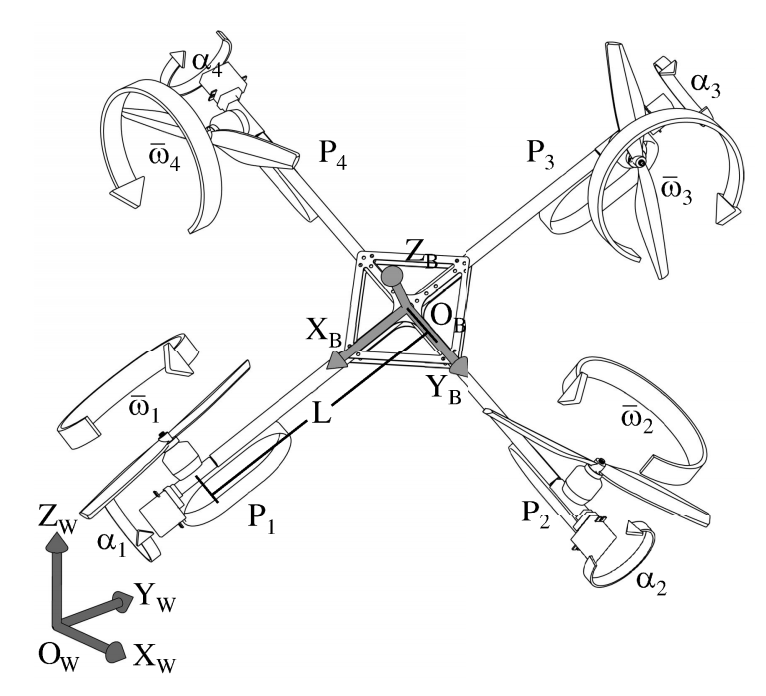
\includegraphics[width=0.65\columnwidth]{ryll_scheme}
	\caption{ -- Общая схема БЛА, расмматриваемого в работе \cite{Ryll01} (рисунок авторов)}
 	\label{fig:ryll_scheme}
\end{figure}
%%%!"!!!!!!!!!!!!!!!!!!!!!!!!!!!!!!!!!!!!

В вектор состояния входят координаты ценра масс аппарата и его ориентация, представленная в матричном виде.
В качестве компонент вектора управляющего воздействия выбраны скорости изменения оборотов двигателей с пропеллерами и скорости поворота двигателей вокруг соответсвующих лучей.
\begin{equation} \label{eq:ryll_ctrl_out}
\begin{aligned}
&\bm{u} = (\dot{\bm \omega}_u,  \dot{\bm \theta}_u)^T,
\\
\bm \omega_u =
(\tilde\omega_1 |\tilde\omega_1|,
\tilde\omega_2 |\tilde\omega_2|&,
\tilde\omega_3 |\tilde\omega_3|,
\tilde\omega_4 |\tilde\omega_4|)^T,
\quad
{\bm \theta}_u = (\theta_1, \theta_2 , \theta_3 , \theta_4 )^T.
\end{aligned}
\end{equation}

Для синтеза контура управления авторы упрощают динамическую модель, принебрегая некоторыми эффектами,
в том числе силой аэродинамического сопротивления, гироскопическими эффектами со стороны корпуса аппарата и роторов с пропеллерами. Преобразованная модель принимает вид
\begin{equation} \label{eq:ryll_dyn}
\begin{aligned}
&\ddot{\bm r}_I = \bm F_g + \frac{1}{m}~^I \bm R_B \bm F(\bm \theta_u) \bm \omega_u,
\\
&\dot {\bm \Omega}_B = \bm J_B \bm T(\bm \theta_u) \bm \omega_u,
\end{aligned}
\end{equation}
где матрицы $\bm F(\bm \theta_u)$ и $\bm T(\bm \theta_u)$ отвечают за текущую геометрию аппарата и с учетом выбранной схемы (рис.\ref{fig:ryll_scheme}) 
\begin{equation} \label{eq:ryl_dyn_matrixes}
\begin{aligned}
&\bm F(\bm \theta) =
\begin{bmatrix}
0&-ks_2&0&ks_4\\
-ks_1&0&ks_3&0\\
kc_1&-kc_2&kc_3&-kc_4
\end{bmatrix},
\\
\phantom{}
\\
&\bm T(\bm \theta) =
\begin{bmatrix}
0&-Lkc_2&0&Lkc_4\\
-Lkc_1&0&Lkc_3&0\\
-Lks_1&Lks_2&-Lks_3&Lks_4
\end{bmatrix}
+
\begin{bmatrix}
0&-bs_2&0&bs_4\\
bs_1&0&-bs_3&0\\
-bc_1&-bc_2&-bc_3&-bc_4
\end{bmatrix}, 
\end{aligned}
\end{equation}
где $c_i = \cos(\theta_i)$, $s_i = \sin(\theta_i)$.
Затем выражения \eqref{eq:ryll_dyn} дифференцируют по времени
\begin{equation} \label{eq:ryll_dyn_dot}
\begin{aligned}
\begin{bmatrix}
&\dddot{\bm r}_I
\\
&\ddot{\bm \Omega}_B
\end{bmatrix}
=
\bm A(\bm \theta_u, \dot {\bm \omega}_u)
\begin{bmatrix}
&\dot{\bm \omega}_u
\\
&\dot{\bm \theta}_u
\end{bmatrix}
+
\bm b(\bm \theta_u, \bm \omega_u, \bm \Omega_B).
\end{aligned}
\end{equation}
Для решения поставленной задачи управления авторы синтезирует регулятор,
\begin{equation} \label{eq:ryll_reg}
\begin{aligned}
\dddot{\bm{r}_d}(t)&=
\dddot{\bm{r}}^0(t) +
\bm{K}_{r1}(\ddot{\bm{r}}^0(t) - \ddot{\bm{r}}(t)) +
\bm{K}_{r2}(\dot{\bm{r}}^0(t) - \dot{\bm{r}}(t)) + 
\bm{K}_{r3}\delta \bm r,
\\
\ddot{\bm{\Omega}_d}(t)&=
\ddot{\bm{\Omega}}^0(t)
+ \bm{K}_{\Omega1}(\dot{\bm{\Omega}}^0(t)-\dot{\bm{\Omega}}(t))
+ \bm{K}_{\Omega2}(\bm{\Omega}^0(t)-\bm{\Omega}(t))
+ \bm{K}_{\Omega3}\delta\bm{R},
\end{aligned}
\end{equation}
сходимость которого обеспечивается выбором матриц коеффициентов $\bm K_{\times}$, которые должны удовлетворять критерию Рауса-Гурвица, а затем обращают динамику и находят вектор $\bm u$, используя псевдообращение Мура-Пенроуза \cite{Barata01}
\begin{equation} \label{eq:ryll_inversed}
\begin{aligned}
\begin{bmatrix}
&\dot{\bm \omega}_u
\\
&\dot{\bm \theta}_u
\end{bmatrix}
=
\bm A^+ \left(
\begin{bmatrix}
&\dddot{\bm r}_I
\\
&\ddot{\bm \Omega}_B
\end{bmatrix}
+
\bm b
\right)
+
(\bm E_8 - \bm A^+ \bm A) \bm \zeta.
\end{aligned}
\end{equation}

Вектор $\bm \zeta$ позволяет использовать две дополнительные степени свободы, возникающих в результате того, что размерность вектора управляющих воздействий превышает размерность вектора состояния, для поддержания ненулевых значений оборотов двигателей, что необходимо для возможности псевдообращения матрицы $\bm A$.

Авторы отмечают, что при реализации обратных связей в контуре управления возможны сложности
с оценкой второй производной текущего положения и ориентации, входящих в регулятор \eqref{eq:ryll_reg},
так как численное дифференцирование сигнала инерциальных датчиков приведет к высокому уровню шума.
Для оценки этих параметров движения предложено воспользоваться выражениями \eqref{eq:ryll_dyn_dot}.
При этом положение, скорость, ориентация и угловая скорость
измеряется с помощью внешней следящей системы,
также на борту обеспечены измерения оборотов двигателей и углов отклонения сервоприводов.

Для уточнения параметров динамики модели авторы проводят ряд измерений, экспериментально уточняя аэродинамические свойства пропеллеров и переходные процессы в сервоприводах, отвечающих за наклон двигателей.

В работе приводятся численные эксперименты, а после исследователи демонстрируют воплощение алгоритмов управления в прототипе.
В качестве траектории выбрана плоская "восьмерка".
Ошибка позиционирования БЛА составила около 5 сантиметров, ориентации -- не более 0,1 радиана.

Основным преимуществом этой работы является детальное рассмотрение управляемой динамики БЛА с поворотными роторами, подробное описание алгоритмов и способов инженерной реализации БЛА такой конструкции.
К недостаткам можно отнести необходимость оценки рывка и углового ускорения в каждый момент времени, а предложенный способ такой оценки, основанный на использовании упрощенной модели \eqref{eq:ryll_dyn_dot} имеет ограничения, связанные с исключением из модели сил аэродинамического сопротивления и гироскопических моментов, что может приводить к значительным ошибкам при некоторых условиях, например, наличии порывов ветра. Другим недостатком является отсутствие реализации строгих ограничений на компоненты вектора управляющих воздействий. Некоторый анализ и дополнения к работе \cite{Ryll01} предложены в исследовании \cite{Stolc01}.

В работе  \cite{Invernizzi01} также рассматривается управляемая динамика квадрокоптера с поворотными роторами. В основе синтеза системы управления лежит ряд геометрических приобразований модели динамики мультироторного робота, для чего пришлось значительно ее упростить.
Для учета ограничений на максимальные углы отклонения поворотных роторов авторы запретили выходить вектору общей тяги аппарата из конусовидной области, параметры которой опредяляются пределами отклонения сервоприводов.
Численные эксперименты показали способность аппарата отслеживать траекторию в виде плоской восьмерки, одновременно меняя свою ориентацию.
При этом углы отклонения сервоприводов не вышли за пределы обозначенных пределов, однако, как сами пояснили авторы, они еще не смогли доказать, что применение такого метода всегда будет гарантировать такой результат.

Еще один пример использования поворотных роторов в конструкции квадрокоптера -- работа \cite{Nemati01}.
Авторы рассматривают аппарат \textit{plus}-конфигурации.
Модель подразумевает возможность симметрично поворачиваться одной паре двигателей.
Авторы применяют метод линеаризаци обратной связи и показывают, что таким образом возможно осуществлять движение и независимо управлять углом тангажа.

Другую техникку для синтеза управления квадрокоптера с поворотными роторами применили в исследовании \cite{Falconi01}.
Замена переменных в модели помогли им численно обратить динамику БЛА и получить выражения для углов отклонения двигателей и оборотов каждого из них, чтобы выход системы соостветсвовад выходу ПД регулятора, который обеспечивает сходимость положения и ориентации БЛА к целевым.
Вычислительные эксперименты показали работоспособность предложенного алгоритма.

Скользящий режим для синтеза контура управления БЛА с поворотными роторами применяется в \cite{Yih01}. 
Численные эксперименты подтвердили способность аппарата перемещаться в точку при неизменной ориентации корпуса.

Исследование маневренных возможностей квадрокоптеров с поворотными роторами с большими пределами отклонений сервоприводов проведено в работе \cite{Oosedo01}.
Показана возможность полета с углами тангажа и рысканья окло 90 градусов.
Проведены летные испытания.

Вычислительно простой способ управления БЛА с поворотными роторами разработан в \cite{Alkamachi01}. Рассмотрена нестандартная схема, где каждый из двигателей может вращаться вокруг луча,
параллельного поперечной оси корпуса аппарата.
Для управления позицией и ориентацией использовались ПИД-регуляторы.
Все роторы наклоняются синхронно.
Контур управления показал хорошую производительность в условиях внешних возмущений, шума измерений и неопределенности в параметрах динамики БЛА.

